\subsection{Benchmarks}

Afin de mesurer les performances de chaque solution, nous avons utilisé un logiciel libre qui se nomme IPPERF

\subsubsection{Configuration d'IPperf}

Le but de ce benchmark est de faire transiter du trafic dans le tunnel VPN. Pour pouvoir effectuer des mesures, IPperf doit être lancé sur une machine cliente et une machine serveur.
Voici le schéma de principe expliquant nos tests de performances:

\begin{figure}[H]
	\begin{center}
		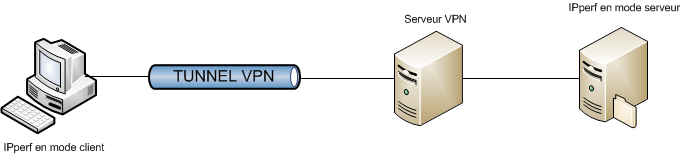
\includegraphics[width=0.75\textwidth]{partie_3/images/ipperf.png}\\
	\end{center}
	\caption{Protocole de test}
	\label{Protocole_de_test}
\end{figure}

Voici la configuration d'IPperf.

En mode serveur:
\verb|iperf.exe -s -i1|

L'option \verb|-s| correspond au mode serveur et le \verb|-i1| correpond à l'intervalle de la prise de mesure (ici notre intervalle est d'une seconde).

En mode client : 
\verb|iperf.exe -c 10.0.1.25 -i1 -t40 |
L'option \verb|-c| correspond au mode client et le \verb|-i1| correpond à l'intervalle de la prise de mesure (ici notre intervalle est d'une seconde), l'option \verb|-t40| permet d'effectuer la mesure sur quarante secondes.

A présent, confrontons les résultats qu'IPperf nous a fournit.

\subsubsection{Confrontration des résultats}

Voici les caractèristiques de la plateforme ayant fait office de serveur:

\begin{figure}[H]
	\begin{center}
\begin{tabular}{|l|c|c|}
\hline
Caractéristiques & Machine \\
\hline
CPU & Intel Core 2 Duo T8100 2,10GHz \\
RAM & 3 Go \\
Carte réseau & Intel 82566MM Gigabit \\
\hline
\end{tabular}
	\end{center}
	\caption{Caractéristique de la plateforme serveur}
	\label{Caractéristique_de_la_plateforme_serveur}
\end{figure}

Concernant les machines clientes, nous avons utilisés les machines présentes dans la salle A214.

Voici les résultats que nous avons obtenus. Le débit trouvé correspond à une moyenne de quarante mesures.

\begin{figure}[H]
	\begin{center}
\begin{tabular}{|l|c|c|c|}
\hline
Solutions & WINDOWS & LINUX & CISCO \\
\hline
Bande Passante(moyenne) & 18Mbps & 50Mbps & 31Mbps \\
Utilisation CPU & 100\% & 80\% & 100\% \\
\hline
\end{tabular}
	\end{center}
	\caption{Résultat des benchmarks}
	\label{Résultat_des_benchmarks}
\end{figure}

Le critère correpondant à l'utilisation CPU n'est pas donné par IPperf. Nous avons seulement regarder les statistiques de la machine. Dès que du trafic passe par le tunnel, les serveurs VPN sont sollicités et il devient très difficile d'exécuter une tâche en parallèle. La surconsommation des ressources machines est dû au processeur.Ce dernier est responsable du traitement des packets transitant dans la carte réseau.

Concernant la bande passante, la solution d'OpenVPN est la plus performante.Cependant, nous avons remarqué des fluctuations durant les mesures, ce qui n'est pas le cas de routeur CISCO.

Après avoir confronter les résultats, faisons le bilan de ces trois solutions.

